%\documentclass[a4paper,KOMA,landscape,titlepage]{powersem}
\documentclass[letterpaper,KOMA,landscape,titlepage]{powersem}
\usepackage[stmo,button]{ifmslide}
\usepackage{graphicx}
%\usepackage{amsmath}
%\usepackage{amsfonts}
%\usepackage{listings}
%\usepackage[T1]{fontenc}
%\usepackage{mathptmx}
%\usepackage{charter}
%\usepackage{pictexwd}

%%%%%%%%%%%%%%%%%%%%%%%%%%%%%%%%%%%%%%%%%%%%%%%%%%%%%%%%%%%%%%%%%%%%
% Set some info on the pdf-file itself (optional)
%%%%%%%%%%%%%%%%%%%%%%%%%%%%%%%%%%%%%%%%%%%%%%%%%%%%%%%%%%%%%%%%%%%%
\hypersetup{pdfauthor={John Sibert}}
\hypersetup{pdfsubject={Assessment Model of MHI YFT Stocks}}
\hypersetup{pdftitle={Assessment model of Main Hawaiian Islands
Yellowfin Tuna Population}}
\hypersetup{pdfkeywords={yellowfin tuna, state space, abundance index, model, Hawaii}}
\hypersetup{pdfpagemode=UseOutlines} %Thumbs}
\hypersetup{bookmarks=true}

\newcommand\doublespacing{\baselineskip=1.6\normalbaselineskip}
\newcommand\singlespacing{\baselineskip=1.0\normalbaselineskip}
\renewcommand\deg[1]{$^\circ$#1}
\newcommand\SD{SEAPODYM}
\newcommand\MFCL{MULTIFAN-CL}
\newcommand\ADMB{ADModel Builder}
\newcommand\SPC{Secretariat of the Pacific Community}
\newcommand\WCPO{Western Central Pacific Ocean}
\newcommand\SSAP{Skipjack Survey and Assessment Programme}
\newcommand\RTTP{Regional Tuna Tagging Programme}
\newcommand\PTTP{Pacific Tuna Tagging Programme}
\newcommand\FAD{fish aggregating device}
\newcommand\ADRM{advection-diffusion-reaction model}
\newcommand\help[1]{\color{red}{\it #1 }\normalcolor}
\newcommand\widebar[1]{\overline{#1}}
\newcommand\EEZ{Exclusive Economic Zone}

\newcommand\None{{N_{1,1}}}
\newcommand\Ntwo{{N_{2,1}}}
\newcommand\Nsum{{N_{1,1}+N_{2,1}}}
\newcommand\peryr{yr$^{-1}$}
\newcommand\prevN[1]{{#1_{t-\Delta t}}}
\newcommand\nextN[1]{{#1_t}}
\newcommand\MSY{\widetilde{Y}}
\newcommand\Fmsy{F_{\MSY}}
\newcommand\MSYFmsy{\MSY\;\Fmsy}
\newcommand\Bd{B_1\; d}

\begin{document}
\pageTransitionReplace
\pagecounter[on]
\slidepagestyle{empty}
\panelposition{outsidebottom}


%\freelogo(25,-13)[1.09cm] % outside bottom right of page counter
\freelogo(25,-13.8)[1.2cm] % outside bottom right of page counter

\definecolor{mytitle}{rgb}{0.0,0.4,0.5}
\definecolor{myauthor}{rgb}{0.9,0.9,0}
\definecolor{section1}{rgb}{0,0,.9}

%%%%%%%%%%%%%%%%%%%%%%%%%%%%%%%%%%%%%%%%%%%%%%%%%%%%%%%%%%%%%%%%%%%%
%\orgname{Universty of Hawaii}
%\orgname{Retirement-failure Consulting}
%\orgurl{http://admb-project.org/}

\author{\scalebox{1}[1.3]{John Sibert, Retirement-failure Consulting}} 
\title{Feasibility of developing a stock assessment model for Main
Hawaiian Islands Yellowfin Tuna Fishery\\
\vspace{4ex}
Part Deux}


\address{\href{mailto:sibert@hawaii.edu}{sibert@hawaii.edu}}

\begin{slide}
\maketitle
\end{slide}
\centerslidesfalse

\begin{slide}\section{Combined HDAR and NOAA Catch Time Series}
\begin{center}
\includegraphics[height=0.8\textheight]{./graphics/5_gear_catch_history_a.pdf}\\
{\Large \bfseries \color{red}{No Recreational Data}\normalcolor}
\end{center}
\end{slide}

\begin{slide}\section{Feasibility questions}
\begin{enumerate}
\item Can we contrive a simple model of the MHI YFT population and
fishery?
\item Can model parameters be estimated from the data?
\item Are biomass estimates plausible?
\item Can model results be used in alphabet soup?
\end{enumerate}
\end{slide}

\begin{slide}\section{Principle model assumptions}
\begin{enumerate}
\item The dynamics of the population of YFT in the MHI follows a
state-space surplus production (Schaefer) model.
\item Fishing mortality exerted by each gear is represented by
distinct random walks with common variance.
\item Predicted catch by gear is the product of estimated fishing mortality
for each gear and average predicted biomass during a year.
\item Optional use of MFCL biomass estimate as index of abundance so
that local abundance is {\bfseries approximately proportional} to the
index biomass.
\end{enumerate}
\end{slide}

\begin{slide}\section{WCPFC Stock Assessments}
\label{fig:MFCL2}
\begin{center}
\begin{tabular}{cc}
MFCL Region 2 & MFCL Region 4\\
\includegraphics[width=0.45\textwidth]{./graphics/annual_region_2_biomass.pdf}&
\includegraphics[width=0.45\textwidth]{./graphics/annual_region_4_biomass.pdf}\\
\end{tabular}
\end{center}
\end{slide}

\begin{slide}\section{Estimabilty}
{\scriptsize
\label{tag:ests4}
\begin{center}
\begin{tabular}{|ll|rr|rr|}
\hline
Index && \multicolumn{2}{c|}{None}&\multicolumn{2}{c|}{MFCL 2}\\
%\cline{3-4}\cline{5-6}
\hline
\multicolumn{2}{|c|}{Parameterization}&$\MSYFmsy$&$\Bd$&$\MSYFmsy$&$\Bd$\\
\multicolumn{2}{|c|}{Designation}& A & B& C& D\\
\hline
\hline
$n$ & Estimated Parameters &4 & 5 & 5 & 6\\
$|G|_{max}$& Gradient at Minimum & $\underline{\mbox{0.0016409}}$ & 33.1289 &
$\underline{\underline{\mbox{3.51082e-05}}}$ & 3.77653\\
$-\log L$& Likelihood & -237.238 & -237.968 & -247.175 & -243.343\\
AIC & Akaike Criterion & -466.476 & -465.936 & -484.350 & -474.686\\
\hline
$B_1$& Initial Biomass & --- & 1184.2 & --- & 2802.3\\
$d$ &$K=dB_1$ & --- & 9.6674 & --- & 2.6348\\
$\MSY$& MSY & 1147.5 & (1199.3) & 1288.7 & (1032.6)\\
$\Fmsy$& F at MSY & 0.82239 & (0.20952) & 0.1668 & (0.2797)\\
$r$& Growth Rate & (1.6448) & 0.41904 & (0.3336) & 0.5594\\
$K$& Equilibrium Biomass & (2790.8) & (11448) & (15452) & (7383.5)\\
$\sigma_P$& Process Error & 0.37416 & 0.36757 & 0.2743 & 0.2649\\
$\sigma_Y$& Observation Error & 0.41693 & 0.43062 & 0.46924 & 0.47614\\
$Q$& Index Proportionality  & --- & --- & 0.04321 & 0.016535\\
\hline
\end{tabular}
\end{center}
}
%\renewcommand{\baselinestretch}{0.1}
%\par{\tiny
%Model estimates from four different model configurations using the
%default prior on $r$.
%Model complexity, expressed in number of parameters estimated ($n$)
%increases from left to right. Long dashes (---) indicate parameters
%not estimated. 
%%$n$ indicates the number of parameters estimated; 
%$-\log L$ is the negative log likelihood (the smaller the number, the
%better the fit);
%$|G|_{max}$ is the curvature of the likelihood at the its apparent
%minimum (values greater than $0.01$ indicate non-convergence).
%%other variables are defined in Table~\ref{tab:allvars1}.
%}
\end{slide}

\begin{slide}\section{Estimated Biomass Trends}
\label{fig:estbiomass}
\begin{center}
\includegraphics[height=0.8\textheight]{./graphics/biomass-array.pdf}
\end{center}
\end{slide}

\begin{slide}\section{Production}
\label{fig:estprod}
\begin{center}
\includegraphics[height=0.8\textheight]{./graphics/production-array.pdf}
\end{center}
\end{slide}


\begin{slide}\section{Alternate forcing: MFCL Region 4}
\label{fig:estr4}
\begin{center}
\begin{tabular}{lr}
\includegraphics[width=0.45\textwidth]{./graphics/r4_est_popB1.pdf}&
\includegraphics[width=0.45\textwidth]{./graphics/r4_est_FB1.pdf}\\
\end{tabular}
\end{center}
\end{slide}

\begin{slide}\section{Conclusions}
\begin{enumerate}
\item Yellowfin catch data from fleets operating in the Main Hawaiian
Islands waters are sufficiently informative to estimate 
{\bfseries relative} biomass trends.
\item An index of abundance is required to estimate 
{\bfseries absolute} biomass;\par
{\bfseries absolute estimates are sensitive to the choice of index
population.}
\item Representing trends in fishing mortality as a random walk is a
convenient and effective approach to accounting for the removal of
biomass from the fish population.
\item Estimates of MSY and F$_{msy}$ are possible, but should not be
used for setting ACLs without further analysis.
\item The prior on $r$ is difficult to assign and probably not required.
\end{enumerate}
\end{slide}

\begin{slide}\section{Next Steps?}
\begin{enumerate}
\item Re-evaluate data: Complete (recreational catch)? Accurate (yellowfin or
bigeye)? Stratified appropriately (quarterly or annual; gear types)?
\item Technical review of model, including statistical assumptions
and computing methods.
\item Review previous work on Hawaiian yellowfin fisheries
\item Review previous uses of production models in tuna fisheries
(to improve $r$ prior).
\item Run simulations to evaluate sensitivity of estimates to
different levels of process and observation error.
\item Test alternative biomass indices, e.g. MHI-specific
SEAPODYM estimates.
\item Compare results to Catch-MSY analysis. 
\item Work within WCPFC assessment process to improve applicability of
WCPFC stock assessments to local requirements.
\end{enumerate}
\end{slide}

\begin{slide}\section{Thanks for your attention}
\begin{center}
%\url{https://github.com/johnrsibert/XSSA.git}
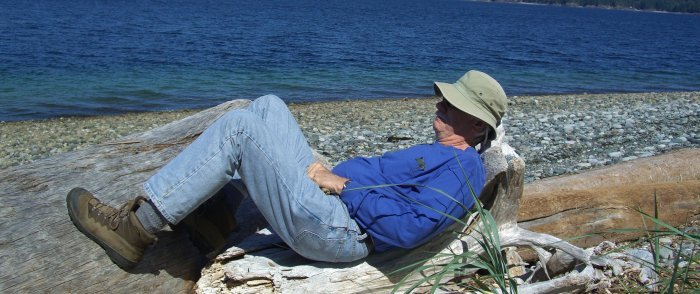
\includegraphics[width=0.8\textwidth]{./graphics/recumbant.png}
\end{center}
\end{slide}

\begin{slide}\section{Technical features}
\begin{enumerate}
\item Fishing mortality and biomass are random effects.
\item All process errors (population growth, fishing
mortality random walk, biomass index proportionality) are assumed
to be equal to a single estimated error $(\sigma_P)$.
\item Zero-inflated log-normal catch likelihood with estimated
observation error $(\sigma_Y)$.
\item Two alternate logistic model parameterizations:
\begin{enumerate}
\item $K = \frac{4\MSY}{r};\quad r = 2\Fmsy$
\item $K = d\cdot B_1$
\end{enumerate}
\item Optional log-normal prior on $r$ with 
$\tilde{r} = 0.486$ and $\sigma_r = 0.8$.
% (Carruthers and McAllister, 2011).
\item Analytic solution to Schaefer ODE for stable propagation
through time.
\end{enumerate}
\vfill
\par Models implemented in ADMB and TMB;
all computer code, data files, and draft reports 
can be found at Github:
\url{https://github.com/johnrsibert/XSSA.git}.
\end{slide}

\begin{slide}\section{Alternative Schaefer Parameterizations}
\begin{center}
%\begin{equation*}
$$\frac{dN}{dt} = rN(1-\frac{N}{K}) - FN$$
%\end{equation}
\end{center}
\begin{itemize}
\item $r=2F_{\MSY};\quad K=\frac{4\MSY}{r}$.
\item Partial non-dimensional: $K=d\cdot B_1$.
\item $K$ as random walk $\log K_t = \log K_{t-1} + \xi_t;\quad \xi_t\sim
N(0,\sigma^2_K)$?
\item $K_t = Q\cdot I_t$?
\item Fully non-dimensional ... ?
\end{itemize}
\end{slide}

\begin{slide}\section{F and Catch Predictions}
\begin{center}
%\includegraphics[height=0.8\textheight]{./graphics/est_catchB1.pdf}
\begin{tabular}{cc}
Fishing Mortality & Catch\\
\includegraphics[width=0.45\textwidth]{../run-issams/use_r_prior/r2/Q1/est_FB1.pdf}
&
\includegraphics[width=0.45\textwidth]{../run-issams/use_r_prior/r2/Q1/est_catchB1.pdf}\\
\end{tabular}

\end{center}
\end{slide}

\begin{slide}\section{Omitting $r$ prior}
\label{tag:ests4NOprior}
{\scriptsize
\begin{center}
\begin{tabular}{|l|rr|rr|}
\hline
Index & \multicolumn{2}{c|}{None}&\multicolumn{2}{c|}{MFCL 2}\\
\cline{2-3}\cline{4-5}
Parameterization&$\MSYFmsy$&$\Bd$&$\MSYFmsy$&$\Bd$\\
Designation& A & B& C& D\\
\hline
\hline
$n$ & 4 & 5 & 5 & 6\\
$-\log L$ & -284.898 & -236.212 & -246.302 & -242.176\\
$|G|_{max}$ & 2.45563 & 151.693 & 1.24795e-05 & 39.9125\\
\hline
$B_1$ & --- & 1540.2 & --- & ---\\
$d$ & --- & 12.567 & --- & ---\\
$\MSY$ & --- & 1274.9 & 1579.3 & ---\\
$\Fmsy$ & --- & 0.13174 & 0.1293 & ---\\
$r$ & --- & 0.26347 & 0.25859 & ---\\
$K$ & --- & 19355 & 24430 & ---\\
$\sigma_P$ & --- & 0.35682 & 0.27044 & ---\\
$\sigma_Y$ & --- & 0.43481 & 0.47162 & ---\\
$Q$ & --- & --- & 0.073752 & ---\\
\hline
\end{tabular}
\end{center} }
\end{slide}

\begin{slide}\section{Posteriors --- Estimated Parameters}
\begin{center}
\includegraphics[width=0.9\textwidth]{./graphics/par_posteriors.pdf}
\end{center}
\end{slide}

\begin{slide}\section{Posteriors --- Functions of Parameters}
\begin{center}
\includegraphics[width=0.9\textwidth]{./graphics/fpar_posteriors.pdf}
\end{center}
\end{slide}


\end{document}
